\documentclass[a4paper]{article}

%% Language and font encodings
\usepackage[english]{babel}
\usepackage[utf8x]{inputenc}
\usepackage[T1]{fontenc}


%% Sets page size and margins
\usepackage[a4paper,top=3cm,bottom=2cm,left=3cm,right=3cm,marginparwidth=1.75cm]{geometry}

%% Useful packages
\usepackage{amsmath}
\usepackage{graphicx}
\usepackage{tikz,pgfplots}
\usepackage[colorinlistoftodos]{todonotes}
\usepackage[colorlinks=true, allcolors=blue]{hyperref}
\usepackage{amsfonts}
\usepackage{bbm}
\usepackage{dsfont}
\usepackage{cancel}
\usepackage{tikz,tkz-base,tkz-fct}
\usepackage{pgfplots}
\newcommand{\prob}{\mathbb{P}}
\newtheorem{definicion}{Definición}
\newtheorem{teorema}{Teorema}
\newtheorem{ejemplo}{Ejemplo}
\DeclareMathOperator*{\argmax}{Arg\,max}
\newtheorem{lem}{Lema}
\newtheorem{prop}{Proposici\'on}
\newtheorem{cor}{Corolario}
\newtheorem{dem}{Demostración}
\numberwithin{equation}{subsection}
\numberwithin{definicion}{subsection}
\newtheorem{obs}{Observación}


%% Aquí se pueden definir nuevas abreviaturas para algunos comandos

\def\sen{{\rm sen\mspace{1.5mu}}}
\def\C{\mathbb C}
\def\R{\mathbb R}
\def\N{\mathbb N}
\def\Q{\mathbb Q}
\def\Z{\mathbb Z}
\def\V{\mathbb V}
\def\E{\mathbb E}
\def\to{\rightarrow}
\newcommand{\pb}{\mathbb{P}}



\newcommand{\ds}{\displaystyle}


%Para hacer normas en tex

\providecommand{\norm}[1]{\lVert#1\rVert}
\providecommand{\normm}[1]{\bigg\lVert#1\bigg\rVert}


%integrales bacanes
\usepackage{ esint }

%Para poner en negrita en modo matemático
\newcommand{\negri}{\boldsymbol}




\title{Simulación Estocástica}
\author{Clase 6}
\date{12 de agosto de 2019}

\begin{document}
\maketitle
\section{Método de Monte Carlo y Simulación}
Para introducir el método de Monte Carlo, consideremos el problema de la integración numérica. Existen diversos métodos numéricos para aproximar (computacionalmente) integrales de la forma:
\[\int_{[0,1]^d}f(x)dx,\]
basados en fórmulas del tipo $\sum_{i=1}^n w_if(x_i)$, cuando $f:\,\R^d\rightarrow\R$ es una función conocida y, usualmente, la suma de los términos $w_i$ es uno y los términos $x_i$ son puntos del conjunto $[0,1]^d$. Por ejemplo, $w_i = 1/k$ y la malla de $[0,1]^d$ compuesta por:
\[\left\{0,\frac{1}{k},\frac{2}{k},\cdots,\frac{k}{k}\right\}^d\hspace{1cm}\text{Para algún $k$ natural.}\]
La cual contiene $n = (k+1)^d$ ($\approx k^d $) puntos. Si el método es de orden 1, el error estará asociado al orden del salto de la malla, en este caso es de $1/k$, por lo tanto:
\[error\,\sim\,\frac{1}{k}\approx \frac{1}{n^{1/d}}\]
Luego, si quisiéramos ajustarnos a un error de un orden pequeño, $\varepsilon > 0$, necesariamente tendríamos que tomar una cantidad de datos proporcionalmente, de la forma; $n\,\approx\,1/\varepsilon^d$, lo que es aceptable para un $\varepsilon$ pequeño y un $d$ pequeño (por ejemplo $d\leq 3$). El problema es que para variables de dimensión mayor a eso, el $n$ asociado crece de manera abrupta. \\Los métodos de Monte Carlos ofrecen una alternativa a este problema, reformulando la integral, vista ahora como la esperanza de una variable aleatoria. La discretización se forma de manera natural al elegir $w_i = 1/n$ y $x_i$ como la realización de variables aleatorias uniformes en $[0,1]^d$. Luego, la convergencia de $\sum_{i=1}^n w_if(x_i)$ estará garantizada por la Ley de los Grandes Números.

\begin{teorema}[Ley de los Grandes Números (L.G.N.)] Sean $(X_n)_{n\in\N}$ variables aleatorias $i.i.d.$, con $\E(X_1)=\mu\,<\,+\infty$. Se define el promedio finito:
\[\overline{X}_n\,=\,\frac{1}{n}\sum_{i=1}^nX_i\]
Entonces:
\[\overline{X}_n\,\xrightarrow{\,\,\,n\,\,\,}\,\mu\hspace{1cm}c.s.\text{ y en }L^1\]
\end{teorema}

\begin{obs}
\begin{itemize}
    \item[]
    \item Si $X_1 \in L^p$, entonces la convergencia es en $L^p$.
    \item Si $\sigma^2 = Var(X_1)\,<\,+\infty$, entonces:
    \[\E\left( \left|\overline{X}_n-\mu\right|\right)\,\leq\,\frac{\sigma}{\sqrt{n}}\]
\end{itemize}
\end{obs}
Además de esto, la taza de convergencia es del orden de $n^{1/2}$ y está dada por el Teorema Central del Límite. Claramente, la taza de convergencia podría parecer algo lenta en comparación con las tazas de otros métodos numéricos de integración en dimensión 1. Pero todos esos métodos colapsan cuando nos escapamos a dimensiones mayores.\newline \\
Siguiendo con el ejemplo anterior, llamemos $I$ a la integral que queríamos aproximar:
\[I\,=\,\int_{[0,1]^d}f(x)dx\]
Si definimos la variable $U\sim\,unif([0,1]^d)$, es decir $U=(U_1,U_2,\cdots,U_d)$, con $U_i\sim\,unif(0,1)$ $i.i.d$, entonces la integral anterior la podemos escribir como $I=\E(f(U))$. Considerando $U^{(1)},U^{(2)},\cdots,U^{(m)}$ realizaciones $i.i.d.$ de la variable $U$, por \textbf{L.G.N.}:
\[\frac{1}{m}\sum_{i=1}^m f(U^{(i)})\,\approx\,I\]

\subsection{Descripción del método}
Para usar el método de Monte Carlo, es necesario poder escribir la cantidad de interes como el valor esperado de una variable aleatoria \textit{"eficientemente simulable en un computador"}. Esto suele ser fácil, como es el caso de la aproximación de una integral, pero podría ganar mucha más complejidad, como cuando deseamos resolver alguna ecuación diferencia parabólica o elíptica.\\ \newline
Sea un valor de interés, $\alpha\in\R$, los pasos a seguir son:
\begin{itemize}
    \item[1.] Escribir $\alpha = \E(X)$, donde $X$ es una variable aleatoria.
    \item[2.] Para algún $n$ suficientemente grande, simular $X_1,X_2,\cdots,X_n$ copias $i.i.d$ de $X$ (muestra).
    \item[3.] Aproximar $\alpha\approx\,\frac{1}{n}\sum_{i=1}^nX_i$.
\end{itemize}
Es calro, por \textbf{L.G.N.} que a medida que nuestra muestra aumenta, la estimación será más cercana. Por lo tanto hay que tener una idea de lo que puede ser "suficientemente grande" en cada caso de estimación.\\
Ventajas de $M.M.C$ (método de Monte Carlo):\\
\begin{itemize}
    \item Simple de implementar.
    \item Escala moderadamente bien, a pesar de la dimensión.
\end{itemize}
Desventajas de $M.M.C$:
\begin{itemize}
    \item El resultado es aleatorio (para cada realización diferente, el resultado de la estimación variará).
    \item El error es del orden $1/\sqrt{n}$, lo que en la practica no suele ser muy bueno.
\end{itemize}
\begin{obs} Si $\sigma^2 = Var(X_1)<\infty$, por el \textbf{T.C.L.}:
\[\frac{\overline{X}_n -\alpha}{\sigma / \sqrt{n}}\approx Z,\hspace{1cm}Z\sim\mathcal{N}(0,1)\]
Así,
\[|\overline{X}_n -\alpha| \approx|Z|\frac{\sigma}{\sqrt{n}}\]
Luego, es de utilidad aproximar (estimar) $\sigma$ para tener una idea del error cometido. 
\end{obs}

\begin{ejemplo}
Dada $Y$ variable aleatoria en $\R$ y $A\subseteq\R$. Si me intereza calcular (estimar):
\[p = \pb\left(Y\in A\right) = \E\left(\mathbbm{1}_{Y\in A}\right)\]
Lo natural es definir $X=\mathbbm{1}_{Y\in A}$. Sean $X_1,X_2,\cdots,X_n$ copias $i.i.d.$ de $X$, luego:
\[p\approx \frac{X_1+X_2+\cdots+X_n}{n}=:\hat{p}\]
Notemos que $\sigma^2 = Var(X) = Var(Bernoulli(p)) = p(1-p) \leq 1/4$ (ver figura).
\newline 
\begin{figure}[h!]
    \centering
    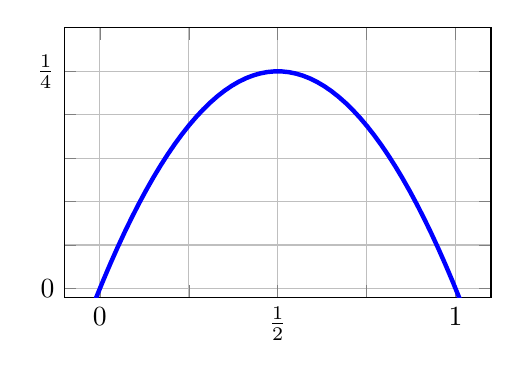
\begin{tikzpicture}
        \begin{axis}[width=7cm, height=5cm,xmin=-0.1,xmax=1.1,ymin=-0.01,ymax=0.3, xmajorgrids=true, ymajorgrids=true, xtick={0,0.25,0.5,0.75,1},  xticklabels={0,,$\frac{1}{2}$,,1}, ytick={0,0.05,0.1,0.15,0.2,0.25}, yticklabels={0,,,,,$\frac{1}{4}$},samples =500]
        \addplot[blue, ultra thick] (x,x-x*x);
        \end{axis}
    \end{tikzpicture}
    \caption{Gráfico de $p(1-p)$, cuyo vértice (punto max) se encuentra en (1/2,1/4)}
\end{figure}\\
Supongamos que queremos un intervalo de confianza al $95\%$, con error $\pm\varepsilon$.
\[0.95 \,\overset{!}{=}\,\pb\left(p\in[\hat{p}-\varepsilon\,,\,\hat{p}+\varepsilon]\right)= \pb\left(|\hat{p}-p|\leq\varepsilon\right) = \pb\left(\frac{|\hat{p}-p|}{\sigma/\sqrt{n}} \leq \frac{\varepsilon\sqrt{n}}{\sigma}\right)\]
Nuevamente, ocupando \textbf{T.C.L.}:
\[0.95\approx \pb\left(|\mathcal{N}(0,1)|\leq \frac{\varepsilon\sqrt{n}}{\sigma}\right)\,\Rightarrow
\,\frac{\varepsilon\sqrt{n}}{\sigma}\approx\,1.96\]
\[\Rightarrow\,\,\sqrt{n}\approx\,\frac{1.96\sigma}{\varepsilon}\,\,\Rightarrow\,\,n\approx\,\frac{1.96^2\sigma^2}{\varepsilon^2}\leq\frac{4\cdot 1/4}{\varepsilon^2}=\frac{1}{\varepsilon^2}\]
Así, ganamos una relación entre la cantidad de muestra que necesitamos para controlar el error asociado a la estimación. Por ejemplo, si queremos un error no mayor a $\varepsilon = 0.01$, bastaría con tomar $n=10000$ observaciones para lograrlo con $95\%$ de confianza.
\end{ejemplo}

\subsection{Simulación de variables aleatorias}
En la actualidad, todos los lenguajes de programación modernos poseen generadores de números \textit{pseudoaleatorios}\footnote{La palabra marca una diferencia respecto al término $aleatorio$, pero no se dará enfoque a este concepto en este curso.}. Tales programas producen como salida, una secuencia perfectamente determinista (y, a veces, periódica), pero cuyas propiedades estadísticas se parecen lo suficiente a las de una secuencia de realizaciones independientes de una variable aleatoria $unif(0,1)$. El problema de crear un "buen generador" de números aleatorios es crear una fórmula de recurrencia que, en un tiempo razonable, produzca una secuencia de números que se parezca lo más posible a una secuencia de realizaciones independientes $unif(0,1)$ con el periodo lo más largo posible.\\ Con este recurso computacional en mente, el objetivo ahora es recreat otras variables aleatorias con distribuciones diferentes que sean de interés, a partir de realizaciones uniformes en el intervalo $(0,1)$.
\end{document}